\graphicspath{{./figures/}}
\title{x86-64 encoding / viruses}
\date{}
\begin{document}
\begin{frame}
    \titlepage
\end{frame}

\begin{frame}{last time}
    \begin{itemize}
    \item x86-64 registers
        \begin{itemize}
        \item overlapping registers
        \item write 32-bit $\rightarrow$ overwrite top of 64-bit
        \item pseudo-register {\tt \%rip}: address of end of instruction
        \item \%xmm/\%ymm registers; x87 floating point stack
        \end{itemize}
    \item AT\&T syntax:
        \begin{itemize}
        \item destination last, \$ for constants (otherwise memory)
        \item \(B,I,S\) $\rightarrow$ $B + I \cdot S$
        \end{itemize}
    \item Linux x86-64 calling convention
    \item lea (load effective address) --- copy address to result
    \item segmentation: {\tt \%fs:0x10}: access 0x10 + base address for FS 
        \begin{itemize}
        \item set by OS, used for thread-local storage
        \end{itemize}
    \end{itemize}
\end{frame}

\begin{frame}{quiz reliability aside}
    \begin{itemize}
    \item appears the quiz site sometimes didn't give \\
        feedback when submitting logged-out of NetBadge
        \begin{itemize}
        \item I don't understand how (200 GET response when there should be NetBadge prompt?)
        \end{itemize}
    \item problem should not recur (quiz submission w/o NetBadge)
    \vspace{.5cm}
    \item let me know if this affected your quiz score
    \end{itemize}
\end{frame}

\section{x86-64 encoding}

\subsection{basics (8 to 32 bit)}
\usetikzlibrary{chains}

\begin{frame}{x86 instruction encoding}
\begin{itemize}
    \item in 2110, 3330 you learned a ``teaching'' machine code
    \item Y86 (3330) is very like what x86 should be
    \item \ldots but it isn't
    \item why? history!
\end{itemize}
\end{frame}

\begin{frame}{the 8086}
\begin{tikzpicture}[overlay,remember picture]
\node[anchor=north east] {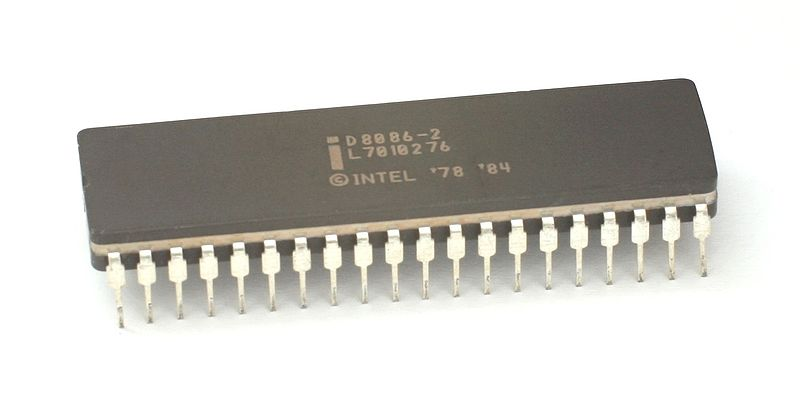
\includegraphics[width=0.3\textwidth]{../x8664-encoding/Intel8086}};
\end{tikzpicture}
\begin{itemize}
    \item 1979 Intel processor
    \item 4 general purpose 16-bit registers: AX, BX, CX, DX
    \item 4 special 16-bit registers: SI, DI, BP, SP
\end{itemize}
\end{frame}

\begin{frame}{8086 instruction encoding: simple}
\begin{itemize}
    \item special cases: 1-byte instructions:
    \begin{itemize}
    \item anything with no arguments
    \item push ax, push bx, push cx, \ldots (dedicated opcodes)
    \item pop ax, \ldots
    \end{itemize}
\end{itemize}
\end{frame}

\begin{frame}{8086 instruction encoding: two-arg}
\begin{itemize}
    \item 1-byte opcode
    \item sometimes {\tt ModRM} byte:
        \begin{itemize}
        \item 2-bit ``mod'' and 
        \item 3-bit register number (source or dest, depends on opcode) and
        \item 3-bit ``r/m'' (register or memory)
        \end{itemize}
    \item ``mod'' + ``r/m'' specify one of:
        \begin{itemize}
        \item {\tt \%reg} (mod = {\tt 11})
        \item {\tt (\%bx/\%bp, \%si/\%di)}
        \item {\tt (\%bx/\%si/\%di)}
        \item {\tt offset(\%bx/\%bp/,\%si/\%di)} (8- or 16-byte offset)
        \end{itemize}
    \item non-intuitive table
\end{itemize}
\end{frame}

\begin{frame}{16-bit ModRM table}
\begin{tikzpicture}
\node (table) {
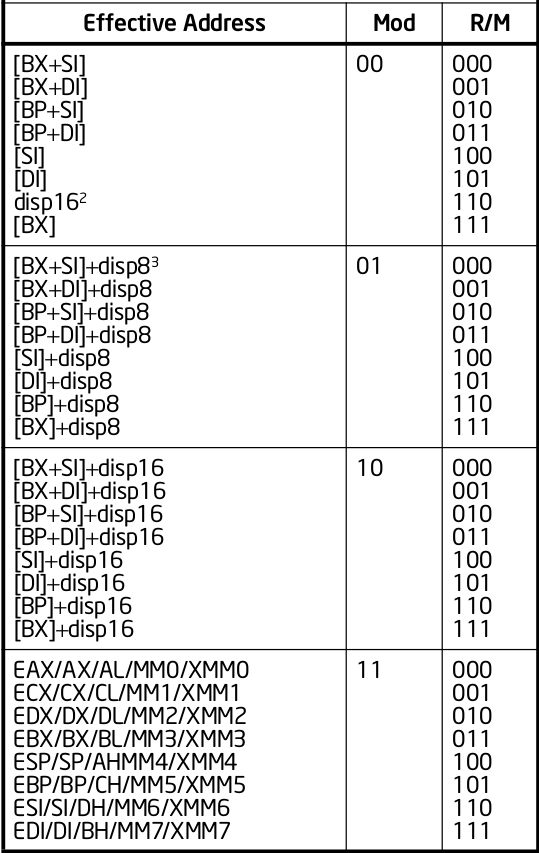
\includegraphics[height=0.8\textheight]{../x8664-encoding/16bitmodrm}
};
\begin{visibleenv}<2>
\node[anchor=north west,align=left] at (table.north east) {
    e.g. \texttt{add \%bl, \%cl} \\
    (Intel syntax: \texttt{add CL, BL}) \\
    Intel manual: \\
    \texttt{02 /r}: \texttt{ADD r8 {\normalfont(dest)}, r/m8} \\
    \texttt{/r} means ModRm byte with reg set to reg\# \\
    ~ \\
    opcode = \texttt{0x02}
    ModRM byte = \\
    \texttt{11} (mod) / \texttt{001} (reg: \%cl) / \texttt{011} (r/m: \%bl) \\
    or \texttt{1100 1011}
    ~ \\
    final encoding: \texttt{02 cb}
};
\end{visibleenv}
\end{tikzpicture}
\end{frame}

\begin{frame}{8086 evolution}
\begin{itemize}
\item Intel 8086 --- 1979, 16-bit registers
\item Intel (80)386 --- 1986, 32-bit registers
\item AMD K8 --- 2003, 64-bit registers
\end{itemize}
\end{frame}

\begin{frame}{x86 modes}
\begin{itemize}
\item x86 has multiple \myemph{modes}
\item maintains compatiblity
\item e.g.: modern x86 processor can work like 8086
    \begin{itemize}
    \item called ``real mode''
    \end{itemize}
\item different mode for 32-bit/64-bit
\item same basic encoding; some sizes change
\end{itemize}
\end{frame}

\begin{frame}{32-bit ModRM table}
\begin{tikzpicture}
\node (table) {
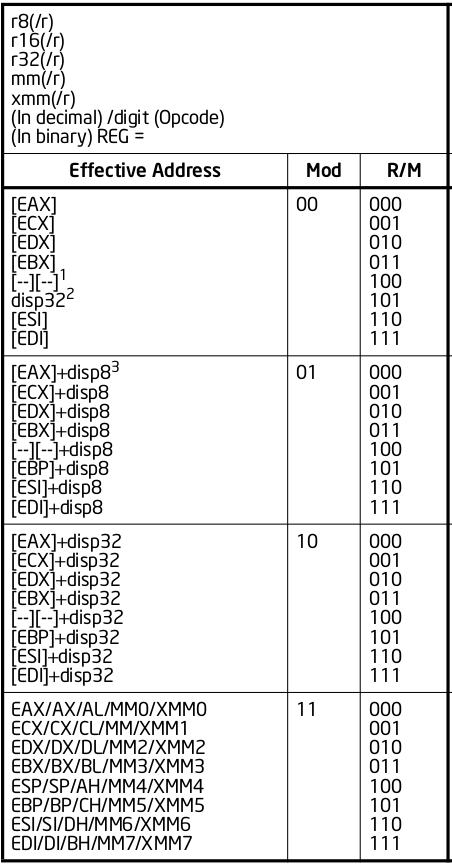
\includegraphics[height=0.8\textheight]{../x8664-encoding/32bitmodrm}
};
\begin{visibleenv}<2>
\node[anchor=north west,align=left] at (table.north east) {
    general pattern for 32-bit x86 register numbering: \\
    AX = 0, CX, DX, BX, SP, BP, SI, DI = 7 \\
    ~ \\
    not all registers treated equally to make space for \\
    special types of addressing: \\
    (base + index * scale, constant address)
};
\end{visibleenv}
\end{tikzpicture}
\end{frame}

\begin{frame}{32-bit addition: SIB bytes}
\begin{itemize}
\item 8086 addressing modes made registers different
\item 32-bit mode got rid of this (mostly)
\item problem: not enough spare bits in {\tt ModRM} byte
\item solution: if ``r/m'' bits = {\tt 100} (4, normally ESP), extra ``SIB'' byte:
    \begin{itemize}
    \item 2 bit \myemph<2>{scale}: {\tt 00} is 1, {\tt 01} is 2, {\tt 10} is 4, {\tt 11} is 8
    \item 3 bit \myemph<3>{index}: index register number
    \item 3 bit \myemph<4>{base}: base register number
    \end{itemize}
\item {\tt (\myemph<4>{\%baseReg},\myemph<3>{\%indexReg},\myemph<2>{scale})}
\end{itemize}
\end{frame}

\begin{frame}{intel manual: SIB table}
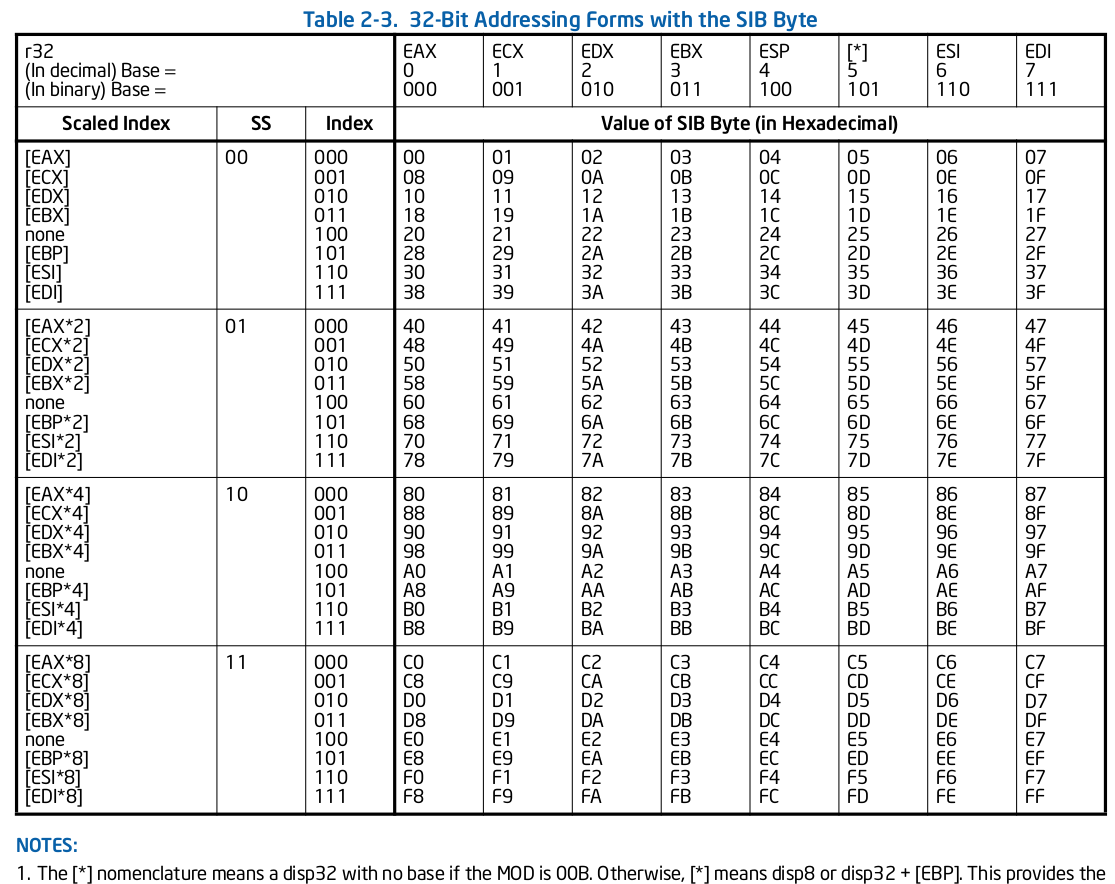
\includegraphics[height=0.9\textheight]{../x8664-encoding/32bitsib}
\end{frame}

\begin{frame}{basic 32-bit encoding}
\begin{tikzpicture}
\begin{scope}[start chain=going right,node distance=0mm,every node/.style={on chain,draw,font=\small,minimum height=1cm}]
\node { opcode }; \node[dashed] { Mod | Reg{\fontsize{9}{10}\selectfont/Opcode} | R/M }; \node[dashed] {SIB byte}; \node[dashed] {displacement}; \node[dashed] {immediate};
\end{scope}
\end{tikzpicture}
\begin{itemize}
\item dashed: not always present
\item opcodes: 1-3 bytes
    \begin{itemize}
    \item some 5-bit opcodes, with 3-bit register field
    \item (alternate view: 8-bit opcode with fixed register)
    \item sometimes Reg part of ModRM used as add'tl part of opcode
    \end{itemize}
\item displacement, immediate: 1, 2, or 4 bytes
    \begin{itemize}
    \item or, rarely, 8 bytes
    \end{itemize}
\end{itemize}
\end{frame}



\subsection{exercise}
\usetikzlibrary{chains}
\begin{frame}{exercise 1} 
\begin{tikzpicture}
\begin{scope}[start chain=going right,node distance=0mm,every node/.style={on chain,draw,font=\small,minimum height=1cm}]
\node (opcode) { opcode }; \node[dashed] { mod | reg{\fontsize{9}{10}\selectfont/opcode} | r/m}; \node[dashed] {scale / idx / base}; \node[dashed] {displacement}; \node[dashed] {immediate};
\end{scope}
\node[anchor=north west] (modrmtbl) at (opcode.south west) {
    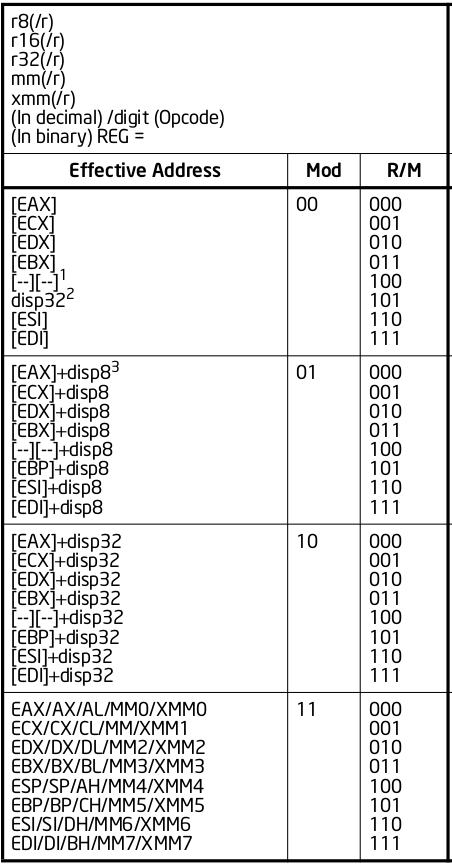
\includegraphics[height=0.8\paperheight]{../x8664-encoding/32bitmodrm}
};
\node[anchor=north west] (bts manual)at (modrmtbl.north east) {
    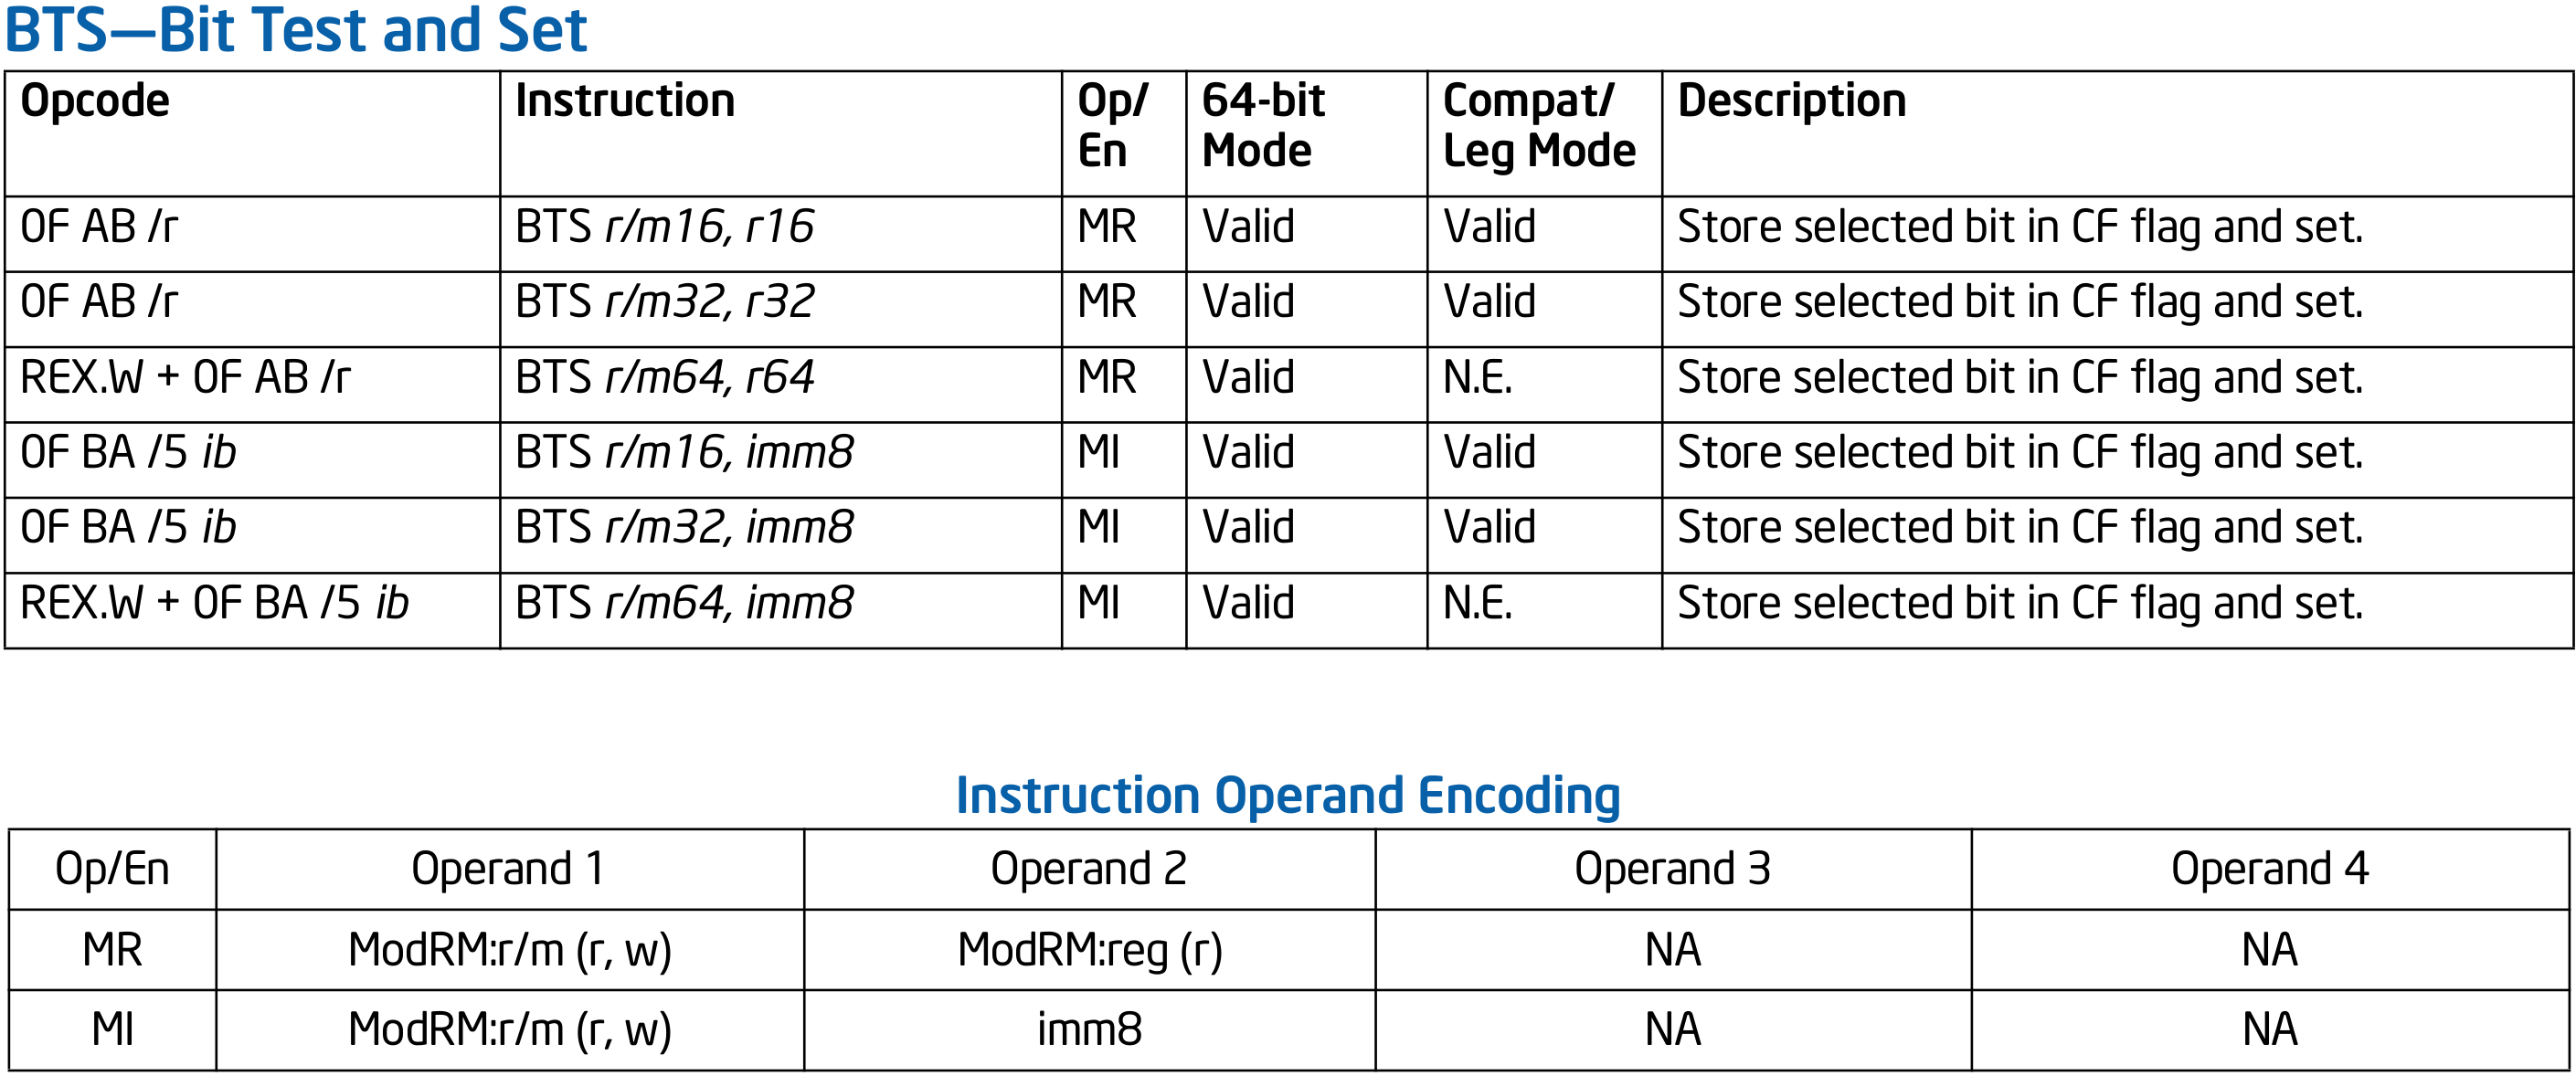
\includegraphics[width=0.75\textwidth]{../x8664-encoding/bts-manual}
};
\node[anchor=north west,align=left] (bts ex) at (bts manual.south west) {
    exercise: encode \texttt{btsl \$7, 4(\%rax)} \\
    (Intel syntax: \texttt{BTS DWORD PTR[RAX+4], 7})
};
\end{tikzpicture}
\end{frame}


\subsection{adding 64-bit}
\usetikzlibrary{arrows.meta,shapes.multipart}

\begin{frame}{what about 64-bit?}
\begin{itemize}
\item adds 8 more registers --- more bits for reg \#?
\item didn't change encoding for existing instructions, so\ldots
\item \myemph{instruction prefix} ``REX''
    \begin{itemize}
    \item 32-bit x86 already had many prefixes
    \end{itemize}
\item also selects 64-bit version of instruction
\end{itemize}
\end{frame}

\begin{frame}{REX prefix}
\begin{tikzpicture}
    \node[draw,rectangle split,rectangle split horizontal, rectangle split parts=5,
        label={north:REX prefix byte}] (rexbyte) {
        {\tt 0100}
        \nodepart{two}
        w
        \nodepart{three}
        r
        \nodepart{four}
        s
        \nodepart{five}
        b
    };
    \node[anchor=north west,align=left] (wExplain) at ([yshift=-5cm,xshift=.5cm]rexbyte.five south) {
        {\tt 1} if 64-bit values ({\tt \%rax}, etc. or from memory)\\
        {\tt 0} if 32-bit values ({\tt \%eax}, etc. or from memory)
    };
    \draw[thick,-Latex] (rexbyte.two south) |- (wExplain.west);
    \node[anchor=south west] (rExplain) at ([yshift=1mm]wExplain.north west) {
        extra bit for ModRM reg field
    };
    \draw[thick,-Latex] (rexbyte.three south) |- (rExplain.west);
    \node[anchor=south west] (sExplain) at ([yshift=1mm]rExplain.north west) {
        extra bit for SIB byte index reg field
    };
    \draw[thick,-Latex] (rexbyte.four south) |- (sExplain.west);
    \node[anchor=south west, align=left] (bExplain) at ([yshift=1mm]sExplain.north west) {
        extra bit for ModRM r/m \\ or SIB base reg field
    };
    \draw[thick,-Latex] (rexbyte.five south) |- (bExplain.west);
\end{tikzpicture}
%\vspace{.5cm}
%\item 4-bit constant 0100
%\item 1-bit ``w'': 1 if 64-bit operands
%\item 1-bit ``r'': extra bit for ModRM register number
%\item 1-bit ``s'': extra bit for SIB index register number
%\item 1-bit ``b'': extra bit for ``r/m'' or SIB index register number 
%    \begin{itemize}
%    \item or modify in-opcode register number
%    \end{itemize}
%\end{itemize}
\end{frame}



\subsection{exercise}
\begin{frame}{64-bit REX exercise (1)}
    \begin{itemize}
    \item \texttt{add \%eax, \%ecx} (Intel: {\tt ADD ecx, eax})
        \begin{itemize}
        \item {\tt 01} (opcode) {\tt c1} (MOD: 11 / REG: 000 (eax) / R\/M: 001 (ecx))
        \end{itemize}
    \item exercise 2a: \texttt{add \%eax, \%r10d} (Intel: {\tt ADD r9d, eax}) = ???
        \begin{itemize}
        \item REX prefix + {\tt 01} + MOD-REG-R/M byte
        \end{itemize}
    \vspace{.5cm}
    \item REX prefix:
        \begin{itemize}
        \item {\tt 0100}
        \item w (is 64-bit values?)
        \item r (extra bit for Reg field)
        \item s (extra bit for SIB index reg)
        \item b (extra bit for R/M or SIB base field)
        \end{itemize}
    \end{itemize}
\end{frame}

\begin{frame}{64-bit REX exercise (2)}
    \begin{itemize}
    \item \texttt{add \%eax, \%ecx} (Intel: {\tt ADD ecx, eax})
        \begin{itemize}
        \item {\tt 01} (opcode) {\tt c1} (MOD: 11 / REG: 000 (eax) / R\/M: 001 (ecx))
        \end{itemize}
    \item exercise 2b: \texttt{add \%rax, \%rcx} (Intel: {\tt ADD rcx, rax}) = ???
        \begin{itemize}
        \item REX prefix + {\tt 01} + MOD-REG-R/M byte
        \end{itemize}
    \vspace{.5cm}
    \item REX prefix:
        \begin{itemize}
        \item {\tt 0100}
        \item w (is 64-bit values?)
        \item r (extra bit for Reg field)
        \item s (extra bit for SIB index reg)
        \item b (extra bit for R/M or SIB base field)
        \end{itemize}
    \end{itemize}
\end{frame}


\subsection{encoding overall}
\begin{frame}{overall encoding}
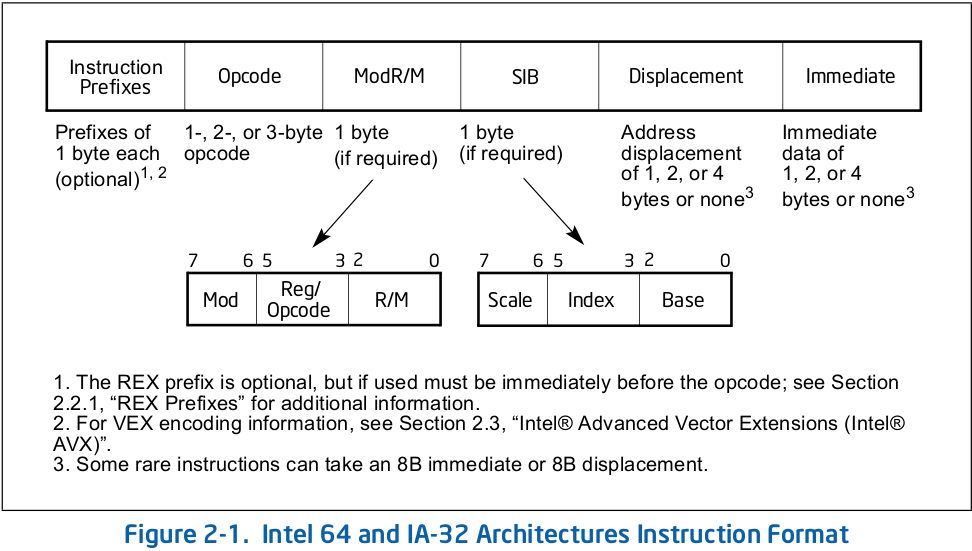
\includegraphics[width=\textwidth]{../x8664-encoding/IntelFig21}
\end{frame}


\subsection{misc prefixes}

\begin{frame}<1>[label=prefixes]{instruction prefixes}
    \begin{itemize}
    \item REX (64-bit and/or extra register bits)
    \item VEX (SSE/AVX instructions; other new instrs.)
    \item operand/address-size change (64/32 to 16 or vice-versa)
    \item {\tt LOCK} --- synchronization between processors
    \item \myemph<2>{{\tt REPNE/REPNZ/REP/REPE/REPZ} --- turns instruction into loop}
    \item segment overrides
    \end{itemize}
\end{frame}




\subsection{examples}

\begin{frame}[fragile,label=x86ex1]{x86 encoding example (1)}
    \begin{itemize}
    \item \lstinline|pushq %rax| encoded as {\tt 50}
        \begin{itemize}
        \item 5-bit opcode {\tt 01010} plus 3-bit register number {\tt 000} \\
        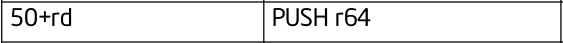
\includegraphics[width=0.4\textwidth]{../x8664-encoding/intel-manual-push-ex1}
        \end{itemize}
    \item \lstinline|pushq %r13| encoded as {\tt 41 55}
        \begin{itemize}
        \item {\tt 41}: REX prefix {\tt 0010} (constant), w:{\tt 0}, r:{\tt 0}, s:{\tt 0}, b:{\tt \color{blue!80!black}{1}}
        \item w = {\tt 0} because push is never 32-bit in 64-bit mode
        \item {\tt 55}: 5-bit opcode {\tt 01010}; 3-bit reg \# {\tt \color{green!80!black}{101}}
        \item 4-bit reg \# {\tt \color{blue!80!black}{1}\color{green!80!black}{101}} = 13
        \end{itemize}
    \end{itemize}
\end{frame}

\begin{frame}[fragile,label=x86ex2]{x86 encoding example (2)}
    \begin{itemize}
    \item \lstinline|addl 0x12345678(%rax,%rbx,2), %ecx|
    \item {\tt 03}: opcode --- add r/m32 into r32 
        \begin{itemize}
        \item
            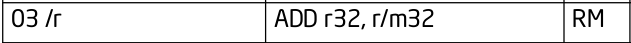
\includegraphics[width=0.4\textwidth]{../x8664-encoding/intel-manual-addl-ex1.png}
            
\includegraphics[width=0.4\textwidth]{../x8664-encoding/intel-manual-addl-ex2.png}
        \end{itemize}
    \item {\tt 8c}: ModRM: mod = {\tt 10}; reg = {\tt 001}, r/m: {\tt 100}
        \begin{itemize}
        \item reg = {\tt 001} = {\tt \%ecx} (table)
        \item SIB byte + 32-bit displacement (table)
        \end{itemize}
    \item {\tt 58}: SIB: scale = {\tt 01}, index = {\tt 011}, base = {\tt 000}
        \begin{itemize}
        \item index {\tt 011} = {\tt \%rbx}; base {\tt 000} = {\tt \%rax};
        \end{itemize}
    \item {\tt 78 56 32 12}: 32-bit constant {\tt 0x12345678}
    \end{itemize}
\end{frame}

\begin{frame}[fragile,label=x86ex3]{x86 encoding example (3)}
    \begin{itemize}
    \item \lstinline|addq 0x12345678(%r10,%r11,2), %rax|
    \item {\tt 4b}: REX prefix {\tt 0100}+w:{\tt \myemph<2>{1}}, r:{\tt \textcolor{violet!80!black}{\myemph<3>{0}}}, s:{\tt \textcolor{blue!80!black}{\myemph<4>{1}}}, b:{\tt \textcolor{green!80!black}{\myemph<5>{1}}}
    \item {\tt 03}: opcode --- add r/m64 to r64 (with \myemph<2>{REX.w})
    \item {\tt 84}: ModRM: mod = {\tt 10}; reg = {\tt 000}, r/m: {\tt 100}
        \begin{itemize}
        \item reg = {\tt \textcolor{violet!80!black}{\myemph<3>{0}}000} = \%rax
        \item SIB byte + 32-bit displacement (table)
        \end{itemize}
    \item {\tt 5a}: SIB: scale = {\tt 01}, index = {\tt 011}, base = {\tt 010}
        \begin{itemize}
        \item with REX: index = {\tt \textcolor{blue!80!black}{\myemph<4>{1}}011} (11), base = {\tt \textcolor{green!80!black}{\myemph<5>{1}}010} (10)
        \end{itemize}
    \item {\tt 78 56 32 12}: 32-bit constant {\tt 0x12345678}
    \end{itemize}
\end{frame}

\begin{frame}[fragile,label=x86ex4]{x86 encoding example (4)}
    \begin{itemize}
    \item \lstinline|movq %fs:0x10,%r13|
    \item {\tt 64}: FS segment override
    \item {\tt 48}: REX: {\tt w}: 1 (64-bit), {\tt r}: \textcolor{violet!80!black}{\tt \myemph<2>{1}}, {\tt s}: \textcolor{blue!80!black}{\tt \myemph<3>{0}}, {\tt b}: \textcolor{green!80!black}{\tt \myemph<4>{0}}
    \item {\tt 8b}: opcode for MOV memory to register
    \item {\tt 2c}: ModRM: mod = {\tt 00}, reg = {\tt 101}, r/m: {\tt 100}
        \begin{itemize}
        \item with REX: reg = {\tt \textbf{\textcolor{violet!80!black}{\myemph<2>{1}}}101} [\%r12]; r/m = {100} (SIB follows)
        \end{itemize}
    \item {\tt 25}: SIB: scale = {\tt 00}; index = {\tt (\textcolor{blue!80!black}{\myemph<3>{0}})100}; base = {\tt (\textcolor{green!80!black}{\myemph<4>{0}})101}
        \begin{itemize}
        \item no register/no register in table
        \end{itemize}
    \item {\tt 10 00 00 00}: 4-byte constant {\tt 0x10}
    \end{itemize}
\end{frame}




\subsection{some impossible instructions}

\begin{frame}[fragile,label=x8664impos]{x86-64 impossibilities}
\lstset{
    language=myasm,
    style=small,
    moredelim={**[is][\sout<all:1>]{~sout~}{~endsout~}},
}
    \begin{itemize}
    \item \myemph{illegal}: \lstinline|~sout~movq 0x12345678ab(%rax), %rax~endsout~|
        \begin{itemize}
        \item maximum 32-bit displacement
        \item \lstinline|movq 0x12345678ab, %rax| okay
            \begin{itemize}
            \item extra {\tt mov} opcode for {\tt \%rax} only
            \end{itemize}
        \end{itemize}
    \item \myemph{illegal}: \lstinline|~sout~movq $0x12345678ab, %rbx~endsout~|
        \begin{itemize}
        \item maximum 32-bit constant
        \item \lstinline|movq $0x12345678ab, %rax| okay
        \end{itemize}
    \item \myemph{illegal}: \lstinline|~sout~pushl %eax~endsout~|
        \begin{itemize}
        \item no 32-bit push/pop in 64-bit mode
        \item but 16-bit allowed (operand size prefix byte {\tt 66})
        \end{itemize}
    \item \myemph{illegal}: \lstinline|~sout~movq (%rax, %rsp), %rax~endsout~|
        \begin{itemize}
        \item cannot use \lstinline|%rsp| as index register
        \item \lstinline|movq (%rsp, %rax), %rax| okay
        \end{itemize}
    \end{itemize}
\end{frame}



\subsection{position-independence} 
\begin{frame}[fragile,label=picVNot]{position dependence}
\begin{itemize}
\item two ways of encoding addresses in x86-64 assembly:
    \begin{itemize}
    \item address in little endian (typically 32-bits --- limit on executable size)
    \item difference between address and \%rip (next instruction address)
    \end{itemize}
\end{itemize}
\hrule
{\tt
\begin{tabular}{l|l}
movb label, \%al & 8a 04 25 {\normalfont\it label's addr (32 bit)} \\
jmp *label & ff 24 25 {\normalfont\it label's addr (32 bit)} \\
movb label(\%rip), \%al & 8a 05 {\normalfont\it \%rip - label's addr (32 bit)} \\
jmp label & e9 {\normalfont\it \%rip - label's addr (32 bit)} \\
\end{tabular}
}
how to know which? --- check manual
\end{frame}


\subsection{PIC: which should be exercise?}
\begin{frame}{position-independence: which to use?}
\begin{itemize}
\item suppose we're inserting ``evil'' code \\
at changing addresses in executable's memory
\item which of the following do we want absolute encoding for? \\
(i.e. which would absolute encoding be easier than relative)
    \begin{itemize}
    \item A. address of a jump from evil code to function at fixed loc in executable
    \item B. address of a jump in a loop in the ``evil'' code
    \item C. address of a string in the ``evil'' code
    \item D. address of a string in the executable
    \end{itemize}
\end{itemize}
\end{frame}




\section{self-replicating malware, generally}

\usetikzlibrary{calc}

\begin{frame}{self-replicating malware}
    \begin{itemize}
    \item attacker's problem: \\getting malware to \myemph{run where they want}
    \item some options:
    \vspace{.5cm}
    \item connect to machine and install it there
    \item send to someone
    \item convince someone else to send it to someone
    \end{itemize}
    \begin{tikzpicture}[overlay,remember picture]
        \begin{visibleenv}<2>
        \node[draw,red!80!black,thick] at ([yshift=1cm]current page.south) {
            \large all automatable!
        };
        \end{visibleenv}
    \end{tikzpicture}
\end{frame}

\begin{frame}<1>{recall: kinds of malware}
    \begin{itemize}
    \item viruses --- infects \myemph{other programs}
    \item \myemph<3>{worms} --- own malicious programs
    \item \myemph<4>{trojans} --- useful (looking) program that also is malicious
    \item \myemph<2>{rootkit} --- silent control of system
    \end{itemize}
    \begin{tikzpicture}[overlay,remember picture]
        \begin{visibleenv}<2>
        \node[draw,red!80!black,thick] at ([yshift=1cm]current page.south) {
            only useful after compromising
        };
        \end{visibleenv}
        \begin{visibleenv}<3>
        \node[draw,red!80!black,thick,align=left] at ([yshift=1cm]current page.south) {
            needs to way to be run in the first place
        };
        \end{visibleenv}
        \begin{visibleenv}<3>
        \node[draw,red!80!black,thick] at ([yshift=1cm]current page.south) {
            targeted ``social engineering''
        };
        \end{visibleenv}
    \end{tikzpicture}
\end{frame}



% FIXME: aside on non-self-replicating malware issues coming up
    % stealth
    % detection

\section{virus: hide in existing programs}

\subsection{motivation}

\begin{frame}{viruses: hiding in files}
    \begin{itemize}
    \item get someone run your malware?
    \item program \myemph{they already want to run}
    \vspace{.5cm}
    \item to spread your malware?
    \item program \myemph<1-2>{they already want to copy}
    \vspace{.5cm}
    \item trojan approach: create/modify new program
    \item simpler: modify already used/shared program
    \end{itemize}
\end{frame}

\begin{frame}{viruses: infecting programs?}
    \begin{itemize}
    \item viruses infecting other programs seems less common
        \begin{itemize}
        \item (but hard to get good statistics\ldots)
        \end{itemize}
    \vspace{.5cm}
    \item but producing infected versions of legitimate software is common
        \begin{itemize}
        \item e.g. fake download site
        \end{itemize}
    \item techniques for automated infection similar to manual infection
    \end{itemize}
\end{frame}


\subsection{early prevalance/motivations}

\begin{frame}[fragile,label=commercial]{virus prevalence}
    \begin{itemize}
        \item viruses \myemph{on commerically sold software media}
        \item from 1990 memo by Chris McDonald:
\begin{Verbatim}[fontsize=\fontsize{8}{9}\selectfont]
4.  MS-DOS INFECTIONS

SOFTWARE                REPORTING LOCATION      DATE     VIRAL INFECTION

a.  Unlock Masterkey    Kennedy Space Center    Oct 89   Vienna
b.  SARGON III          Iceland                 Sep 89   Cascade (1704)
c.  ASYST RTDEMO02.EXE  Fort Belvoir            Aug 89   Jerusalem-B
d.  Desktop Fractal     Various                 Jan 90   Jerusalem (1813)
	Design System
e.  Bureau of the       Government Printing     Jan 90   Jerusalem-B
    Census, Elec. County   Office/US Census Bureau
    & City Data Bk., 1988
f.  Northern Computers  Iceland                 Mar 90   Disk Killer
    (PC Manufacturer shipped infected systems.)
5.  MACINTOSH INFECTIONS

    SOFTWARE            REPORTING LOCATION      DATE     VIRAL INFECTION

a.  NoteWriter          Colgate College         Sep 89   Scores and nVIR
.......
\end{Verbatim}
    \end{itemize}
\imagecredit{https://groups.google.com/forum/\#!original/comp.virus/XJCfYR9T6nI/azflHz5goooJ}
\end{frame}


\begin{frame}{early virus motivations}
    \begin{itemize}
        \item lots of (but not all) early virus software was ``for fun''
        \item not trying to monetize malware
            \begin{itemize}
            \item (like is common today)
            \end{itemize}
        \item hard: Internet connections uncommon
    \end{itemize}
\end{frame}





\section{case study: Vienna}
% FIXME: before introduction to executable formats?


\begin{frame}{Case Study: Vienna Virus}
\begin{itemize}
    \item Vienna: virus from the 1980s
    \item This version: published in Ralf Burger, ``Computer Viruses: a high-tech disease'' (1988)
    \item targetted COM-format executables on DOS
\end{itemize}
\end{frame}




\subsection{aside: COM files}


\begin{frame}{Diversion: .COM files}
    \begin{itemize}
    \item .COM is a \myemph{very simple} executable format
    \item no header, no segments, no sections
    \item file contents loaded at fixed address {\tt 0x0100}
    \item execution starts at {\tt 0x0100}
    \item everything is read/write/execute (no virtual memory)
    \end{itemize}
\end{frame}




\subsection{entry/exit}

\usetikzlibrary{calc}

\begin{frame}[fragile,label=vienna]{Vienna: infection}
\lstset{
    language=myasm,
    style=smaller,
    moredelim={**[is][\btHL<2>]{~hi2~}{~endhi2~}},
}
\begin{tikzpicture}
\tikzset{programBox/.style={draw,thick},every label/.style={inner sep=1mm,outer sep=0mm}}
\node[programBox,minimum height=3cm,label={north:uninfected},anchor=north west] (uninfect) at (0,0) {
\begin{lstlisting}
0x0100:
    ~hi2~mov $0x4f28, %cx~endhi2~
    /* b9 28 4f */
0x0103:
    mov $0x9e4e, %si
    /* be 4e 9e */
    mov %si, %di
    push %ds
    /* more normal
       program
       code */
....
0x0700: /* end */

\end{lstlisting}
};
\node[overlay,programBox,anchor=north west,label={[overlay]north:infected}] at ([yshift=.5cm,xshift=1cm]uninfect.north east) {
\begin{lstlisting}
0x0100: jmp 0x0700
0x0103: mov $0x9e4e, %si
...
0x0700:
    push %cx
    ... // %si <- 0x903
    mov $0x100, %di
    mov $3, %cx
    rep movsb
    ...
    mov $0x0100, %di
    push %di
    xor %di, %di
    ret
...
0x0903:
    ~hi2~.bytes 0xb9 0x28 0x4f~endhi2~
...
\end{lstlisting}
};
\end{tikzpicture}
\end{frame}

\begin{frame}[fragile,label=viennaFixup]{Vienna: ``fixup''}
\lstset{
    language=myasm,
    style=small,
    moredelim={**[is][\btHL<2>]{~hi2~}{~endhi2~}},
    moredelim={**[is][\btHL<3>]{~hi3~}{~endhi3~}},
}
\begin{lstlisting}
0x0700:
    push %cx // initial value of %cx matters??
    mov ~hi3~$0x8fd~endhi3~, %si // %si <- beginning of data
    mov %si, %dx // save %si
        // movsb uses %si, so
        // can't use another register
    add $0xa, %si // offset of saved code in data
    mov $0x100, %di // target address
    mov $3, %cx // bytes changed
    /* copy %cx bytes from (%si) to (%di) */
    rep movsb 
    ...
...
// saved copy of original application code
0x903: ~hi2~.byte 0xb9 .byte 0x28 .byte 0x4f~endhi2~
\end{lstlisting}
\end{frame}

\begin{frame}[fragile,label=viennaReturn]{Vienna: return}
\lstset{language=myasm,style=small}
\begin{lstlisting}
0x08e7:
    pop %cx // restore initial value of %cx, %sp
    xor %ax, %ax // %ax <- 0
    xor %bx, %bx
    xor %dx, %dx
    xor %si, %si
    // push 0x0100
    mov $0x0100, %di
    push %di 
    xor %di, %di // %di <- 0
    // pop 0x0100 from stack
    // jmp to 0x0100
    ret 
\end{lstlisting}
\begin{itemize}
\item<1> question: why not just jmp 0x0100 ?
\end{itemize}
\end{frame}



\subsection{infection outline}


\begin{frame}<1>[label=viennaOutline]{Vienna: infection outline}
\begin{itemize}
\item Vienna \myemph{appends} code to infected application
\vspace{.5cm}
\item \myemph<2>{where does it read the code come from?}
\item \myemph<3>{how is code adjusted for new location in the binary?}
    \begin{itemize}\item what linker would do\end{itemize}
\item \myemph<4>{how does it keep files from getting infinitely long?}
\end{itemize}
\end{frame}


\subsection{writing your own code?}

\againframe<2>{viennaOutline}
\subsubsection{aside: quines}


\begin{frame}{quines}
\begin{itemize}
    \item exercise: write a C program that outputs its source code
        \begin{itemize}
        \item (pseudo-code only okay)
        \end{itemize}
    \item possible in any {\small (Turing-complete)} programming language
    \item called a ``quine''
\end{itemize}
\end{frame}

\begin{frame}[fragile,label=quineClever]{clever quine solution}
\lstset{language=C,style=small,
    moredelim={**[is][\btHL<2|handout:0>]{@hi2@}{@endhi@}},
    moredelim={**[is][\btHL<3|handout:0>]{@hi3@}{@endhi@}},
    showstringspaces=false,
}
\begin{lstlisting}
#include <stdio.h>
char*x="int main(){
       `\btHL<2>{printf(p,10,34,x,34,10,34,p,34,10,x,10);}`
       }";
@hi3@char*p@endhi@="#include <stdio.h>%c
    char*x=%c%s%c;%cchar*p=%c%s%c;
    %c%s%c";
int main(){
    @hi2@printf(p,10,34,x,34,10,34,p,34,10,x,10);@endhi@
}
\end{lstlisting}
\begin{itemize}
\item some line wrapping for readability --- shouldn't be in actual quine
\end{itemize}
\begin{tikzpicture}[overlay,remember picture]
    \begin{visibleenv}<2|handout:0>
        \node[fill=white,draw,thick,align=left] at (current page.center) {
            {\tt printf} to fill template: \\
            {\tt 10} = newline; {\tt 34} = double-quote; \\
            {\tt x}, {\tt p} = template/constant strings
        };
    \end{visibleenv}
    \begin{visibleenv}<3|handout:0>
        \node[fill=white,draw,thick,align=left] at ([yshift=1cm]current page.center) {
            template filled by printf
        };
    \end{visibleenv}
\end{tikzpicture}
\end{frame}

\begin{frame}[fragile,label=quineDumb]{dumb quine solution}
\begin{lstlisting}[language=C,style=small]
#include <stdio.h>
int main(void) {
    char buffer[1024];
    FILE *f = fopen("quine.c", "r");
    size_t bytes = fread(buffer, 1,
                         sizeof(buffer), f);
    fwrite(buffer, 1, bytes, stdout);
    return 0;
}
\end{lstlisting}
\begin{itemize}
\item a lot more straightforward!
\item but ``cheating''
\end{itemize}
\end{frame}




\subsubsection{Vienna replication code}


\begin{frame}[fragile,label=virusWriting]{Vienna copying}
\lstset{
    style=small,
    language=myasm,
    moredelim={**[is][\btHL<2|handout:0>]{@hi2@}{@endhi@}},
}
\begin{lstlisting}
@hi2@mov $0x8f9, %si@endhi@ // %si = beginning of virus data
...
mov $0x288, %cx // length of virus
mov $0x40, %ah  // system call # for write
mov %si, %dx
sub $0x1f9, %dx // %dx = beginning of virus code
int 0x21 // make write system call
\end{lstlisting}
\end{frame}




% FIXME: work through cavaties in loaded stuff not used on ELF 

\end{document}
